% Fourier Optics Lab Report (publication-style)
% Course constraint:
%   - Main narrative <= 4 pages (figures/tables excluded by course rule)
%   - Use ONLY images provided in the uploaded materials
% Author note:
%   - Bold the submitting student's name; list partners in plain text.

\documentclass[10pt,twocolumn]{article}

\usepackage[margin=0.85in]{geometry}
\usepackage{graphicx}
\usepackage{amsmath,amssymb}
\usepackage{siunitx}
\usepackage{booktabs}
\usepackage{microtype}
\usepackage{hyperref}
\usepackage{caption}
\usepackage{subcaption}
\usepackage{float}
\usepackage{enumitem}
\usepackage{placeins}
\usepackage{dblfloatfix}

% ----------------------------
% Layout tuning (reduce white space)
% ----------------------------
% Avoid large inter-paragraph/item stretching that can create big blank regions
% in two-column pages with uneven content.
\raggedbottom

% Top-align floats on float pages (LaTeX otherwise centers them vertically,
% which can leave large blank areas above/between figures).
\makeatletter
\setlength\@fptop{0pt}
\setlength\@fpsep{8pt}
\setlength\@fpbot{0pt}
\setlength\@dblfptop{0pt}
\setlength\@dblfpsep{8pt}
\setlength\@dblfpbot{0pt}
\makeatother

% Slightly tighter default float spacings.
\setlength{\textfloatsep}{10pt plus 2pt minus 2pt}
\setlength{\floatsep}{8pt plus 2pt minus 2pt}
\setlength{\intextsep}{8pt plus 2pt minus 2pt}

\hypersetup{colorlinks=true, linkcolor=blue, citecolor=blue, urlcolor=blue}
\captionsetup{font=small,labelfont=bf}
\setlength{\columnsep}{0.25in}
\setlist[itemize]{leftmargin=*, itemsep=2pt, topsep=2pt}
\setlist[enumerate]{leftmargin=*, itemsep=2pt, topsep=2pt}

\sisetup{
  separate-uncertainty=true,
  per-mode=symbol,
  detect-weight=true,
  detect-family=true
}

\title{Fourier-Plane Metrology, Abbe-Limited Resolution, and Dark-Field Imaging in a 4\,$f$ Microscope}

% NOTE: edit partner list if needed.
\author{\textbf{Hongyu Wang}\\(with Maya Kang-Chou and Sidharth Kannan)\\Department of Physics, University of California, Santa Barbara}
\date{\today}

\begin{document}

\twocolumn[
\maketitle
\begin{abstract}
Access to the objective back focal plane (the \emph{Fourier plane}) in a 4\,$f$ microscope enables both spatial-frequency metrology and Fourier-domain image filtering. Using the Thorlabs EDU-FOP2 kit with a green bandpass filter (nominal $\lambda\approx\SI{550}{\nano\meter}$), we performed the three manual \S2.5 experiments: (1) measured the period of a diffraction grating by (i) screen-angle geometry, (ii) a calibrated camera image, and (iii) Fourier-plane slit cutoff; (2) tested Abbe's diffraction-limited resolution condition (manual Eq.~36) using \SI{4}{\micro\meter} (F1) and \SI{6}{\micro\meter} (F2) lattices; and (3) compared bright-field and dark-field diatom images using a zero-order blocking mask.

The grating period estimates were $d_{\mathrm{screen}}=\SI{9.87\pm0.26}{\micro\meter}$, $d_{\mathrm{cam}}=\SI{9.92\pm0.11}{\micro\meter}$, and $d_{\mathrm{slit}}=\SI{10.83\pm0.05}{\micro\meter}$, where uncertainties denote \emph{random} (repeatability-limited) components.
\emph{Random uncertainty} refers to stochastic variations from readout noise, finite pixel/counting resolution, and repeated alignment that can be reduced by averaging, while \emph{systematic uncertainty (``systematics'')} refers to repeatable biases that do \emph{not} average down (e.g., wavelength error, calibration scale-factor bias, slit mis-centering, or subjective ``just-visible'' thresholds). Comparing methods, the calibrated-camera approach provides the most defensible overall estimate because it uses a traceable object-plane length calibration and a threshold-free period count; the slit method achieves a smaller \emph{random} error but is dominated by systematics, consistent with its $\sim\SI{0.9}{\micro\meter}$ offset.

Using $D=\SI{25.4}{\milli\meter}$ and $f=\SI{150}{\milli\meter}$ gives $\mathrm{NA}\approx0.085$ and $\Delta x_{\min}\approx\SI{4.0}{\micro\meter}$, consistent with the observed stronger suppression of higher diffraction orders for F1 than F2. Zero-order blocking produces dark-field diatom images with enhanced edge contrast, demonstrating Fourier-plane high-pass filtering.
\end{abstract}
\vspace{0.15in}
]

\section{Introduction}
A thin lens performs a Fourier transform: in the paraxial approximation, the complex field in the back focal plane of a lens is proportional to the spatial-frequency spectrum of the field in the front focal plane. In microscopy this implies that an objective separates diffraction orders (spatial frequencies) in its back focal plane. A 4\,$f$ microscope (objective + tube lens separated by $f_{\rm obj}+f_{\rm tube}$) therefore provides two complementary planes: an image plane for direct observation, and a Fourier plane where masks implement spatial-frequency filtering.

The EDU-FOP2 \S2.5 experiments probe three core consequences: (i) the mapping between an object's period and the separation of its diffraction orders (metrology), (ii) the numerical-aperture-limited cutoff of transmitted spatial frequencies (Abbe limit), and (iii) the modification of image contrast by selectively removing low or high spatial frequencies (bright-/dark-field).

\section{Theory}
\subsection{Grating orders and Fourier-plane scaling}
A periodic object of period $d$ produces diffraction orders at spatial frequencies $u_n=n/d$. In an objective Fourier plane, orders appear at transverse positions
\begin{equation}
 x_n = n\,\frac{f_{\rm obj}\,\lambda}{d}\qquad(n\in\mathbb{Z}),
 \label{eq:xn}
\end{equation}
so adjacent-order spacing satisfies the ``uncertainty relation'' (manual Appendix B / writeup)
\begin{equation}
 d\,\Delta x = f_{\rm obj}\,\lambda,\qquad \Delta x\equiv x_{n+1}-x_n.
 \label{eq:uncertainty}
\end{equation}
In the far field, the same physics appears as the grating equation
\begin{equation}
 d\,\sin\theta_m=m\lambda\quad(m=0,\pm1,\pm2,\dots).
 \label{eq:grating}
\end{equation}

\subsection{Abbe / Rayleigh resolution}
The manual's Abbe-style condition (Eq.~36) is
\begin{equation}
\Delta x_{\min}=0.61\,\frac{\lambda}{\mathrm{NA}},\qquad \mathrm{NA}=n\sin\alpha.
\label{eq:abbe}
\end{equation}
We estimate $\sin\alpha$ from the limiting aperture diameter $D$ and focal length $f$ via $\sin\alpha\approx D/(2f)$.

\subsection{Bright-field vs dark-field for weak objects}
A weak phase object transmits a large undiffracted (zero-order) component plus smaller scattered components (higher orders). In bright-field, the zero-order term dominates the background. In dark-field, blocking the zero order suppresses the background and the image is formed primarily from scattered light, emphasizing edges/high spatial frequencies.

\section{Experimental methods}
\subsection{Apparatus, accessible planes, and calibration rationale}

\begin{figure*}[t]
\centering
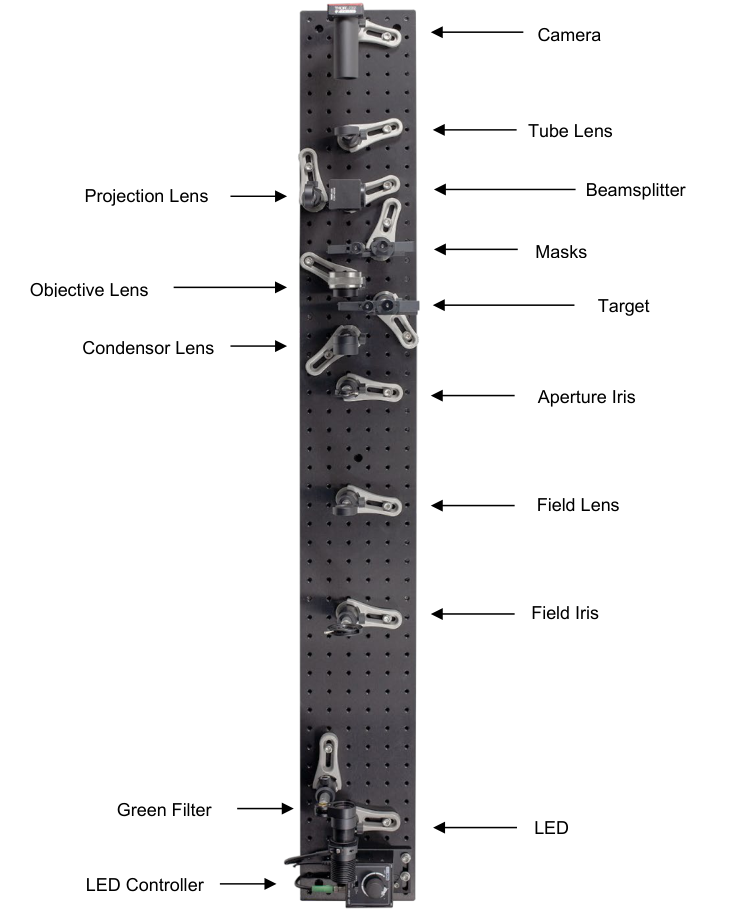
\includegraphics[height=0.78\textheight]{images/manual_setup_fig55.png}
\caption{Overall layout of the Fourier optics kit (reproduced from the provided Thorlabs EDU-FOP2 manual). Masks (including a variable slit) are inserted at an objective Fourier plane, enabling direct control of transmitted spatial frequencies. The camera views the image plane through the tube lens.}
\label{fig:setup}
\end{figure*}

Figure~\ref{fig:setup} is the working ``wiring diagram'' of the experiment. The LED source is filtered to green to approximate monochromatic illumination; this reduces wavelength-dependent systematics in Eqs.~\eqref{eq:xn}--\eqref{eq:abbe}. The field iris and field lens define the illuminated region on the target (K\"ohler-like illumination), while the aperture iris controls the illumination cone and the effective numerical aperture. The condenser lens delivers the illumination onto the target. The objective lens performs the Fourier transform and physically exposes its back focal plane, where diffraction orders become spatially separated and where masks/slits can be inserted. A beamsplitter provides simultaneous access to (i) the image plane (tube lens + camera) and (ii) a relay of the Fourier plane (projection lens + screen).

\begin{figure}[H]
\centering
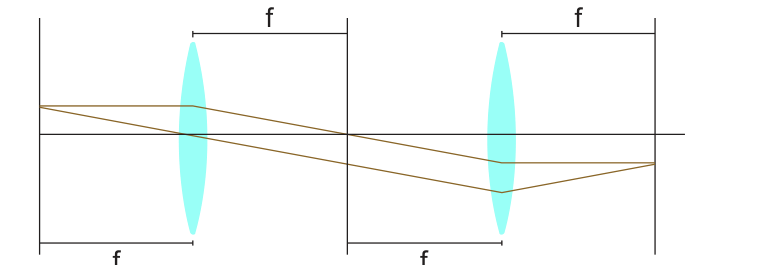
\includegraphics[width=0.95\linewidth]{images/manual_4f_diagram4.png}
\caption{Idealized 4\,$f$ microscope geometry (reproduced from the provided Thorlabs EDU-FOP2 manual). The objective back focal plane is the Fourier plane used for spatial filtering; the tube lens forms a real image on the camera.}
\label{fig:4f}
\end{figure}

Figure~\ref{fig:4f} motivates our three measurement strategies for the grating period. The screen-angle method uses Eq.~\eqref{eq:grating}; the camera method uses an object-plane length calibration to convert pixel counts into $d$; and the slit cutoff method uses the Fourier-plane spacing in Eq.~\eqref{eq:xn} and the ``uncertainty relation'' in Eq.~\eqref{eq:uncertainty}.

\textbf{Alignment procedure (implemented).} We placed the objective behind the condenser with their focal planes overlapped, positioned the tube lens $\sim\SI{18}{-}\SI{20}{\centi\meter}$ above the objective, and adjusted focus until target features were sharp on the camera. We then swapped in the grating or diatom sample without changing lens separations, minimizing changes in conjugate planes.

\textbf{Why camera calibration is required.} For camera-based metrology we need a pixel-to-length conversion \emph{in the object plane}. The camera sensor pixel pitch is not directly relevant because the imaging optics introduce magnification. We therefore imaged a target with a known feature spacing (\SI{0.74}{\milli\meter}) placed in the same plane as the grating; this makes the camera method traceable and reduces systematics.

\subsection{Experiment 1: grating period in three ways}
\textbf{(i) Screen-angle method.} We varied the screen distance $L$ and measured the transverse separation $y$ between the 0th and 1st orders; fitting $y/L$ yields $\tan\theta$, and Eq.~\eqref{eq:grating} gives $d$.

\textbf{(ii) Calibrated camera image.} We obtained an object-plane scale factor $s$ (\si{\micro\meter\,px^{-1}}) from the calibration target, then measured $d=sN/P$ by counting $P$ grating periods across $N$ pixels.

\textbf{(iii) Fourier-plane slit cutoff.} We placed a variable slit in the objective Fourier plane. For a 2D lattice, reducing the slit width blocks first orders along one axis and the image appears one-dimensional. If the slit is centered on the 0th order, the ``just-transmit'' condition is $w_{\min}/2\approx x_1$; combining with Eq.~\eqref{eq:xn} gives
\begin{equation}
 d\approx \frac{2f_{\rm obj}\lambda}{w_{\min}}.
 \label{eq:slit}
\end{equation}

\subsection{Experiment 2: Abbe resolution test}
Using Eq.~\eqref{eq:abbe} and the kit parameters ($D=\SI{25.4}{\milli\meter}$, $f=\SI{150}{\milli\meter}$, $n\approx1$), we predicted $\Delta x_{\min}$ and compared diffraction patterns for two lattices (F1: \SI{4}{\micro\meter}, F2: \SI{6}{\micro\meter}).

\subsection{Experiment 3: bright-field and dark-field diatom images}
We imaged a diatom sample in bright-field (no mask) and then inserted a Fourier-plane mask that blocks the central (zero-order) maximum to obtain a dark-field image.

\FloatBarrier
\section{Results and analysis}
\subsection{Experiment 1: grating period (three methods)}
All raw measurements (and assigned uncertainties) are reported in Appendix~\ref{app:raw}. Full uncertainty propagation is provided in Appendix~\ref{app:calc}.

\textbf{(i) Screen-angle method.} A through-origin regression (constraint $y\to0$ as $L\to0$) gives $\tan\theta=(5.58\pm0.15)\times10^{-2}$ and $\theta=0.0558\pm0.0015\,\mathrm{rad}$. With $m=1$ and $\lambda=\SI{550}{\nano\meter}$,
\begin{equation}
 d_{\mathrm{screen}}=\frac{\lambda}{\sin\theta}=\SI{9.87\pm0.26}{\micro\meter}.
\end{equation}
The dominant random contribution is the manual measurement of $y$ on the viewing screen.

\textbf{(ii) Calibrated camera method.}
\begin{figure}[H]
\centering
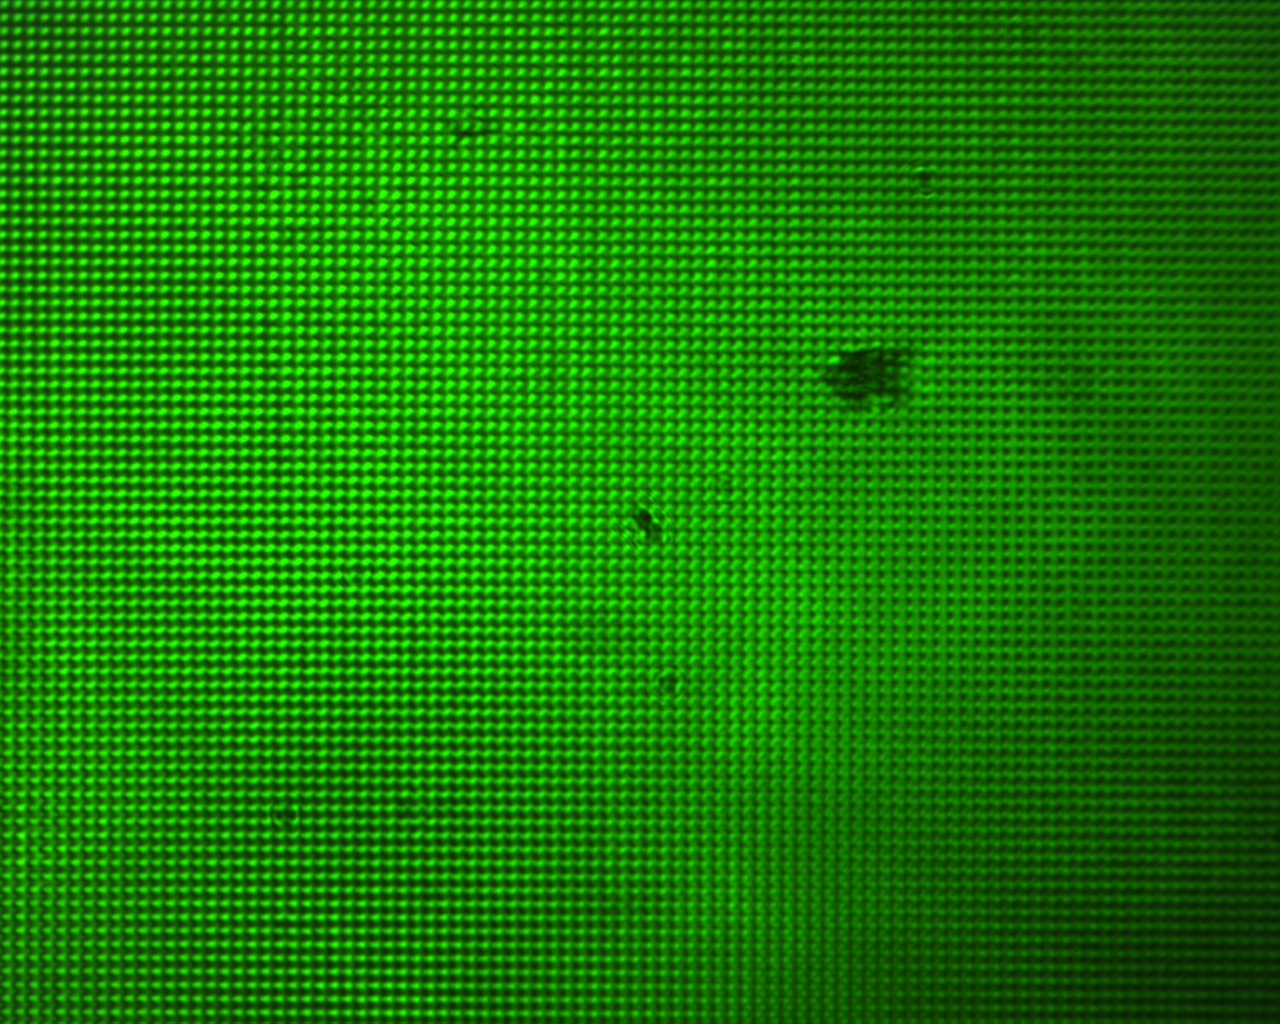
\includegraphics[width=0.92\linewidth]{images/untitled_p2_img1.png}
\caption{Camera image of the diffraction grating (provided lab image) used for the calibrated-camera period measurement. We counted $P=94\pm1$ periods across $N=1280$ pixels in a representative row after aligning the grating to minimize tilt.}
\label{fig:grating_img}
\end{figure}

Figure~\ref{fig:grating_img} illustrates the key advantage of the camera method: once the object-plane scale $s$ is calibrated, the period estimate reduces to a discrete count that is relatively insensitive to subjective thresholds. The calibration factor was
\begin{equation}
 s=\frac{\SI{0.74}{\milli\meter}}{1016\pm2\,\mathrm{px}}=\SI{0.728\pm0.001}{\micro\meter\,px^{-1}},
\end{equation}
so that
\begin{equation}
 d_{\mathrm{cam}}=\frac{sN}{P}=\SI{9.92\pm0.11}{\micro\meter}.
\end{equation}

\textbf{(iii) Fourier-plane slit cutoff.} With $f_{\rm obj}=\SI{30}{\milli\meter}$ and $w_{\min}=\SI{0.1200\pm0.0005}{in}=\SI{3.048\pm0.013}{\milli\meter}$,
\begin{equation}
 d_{\mathrm{slit}}=\frac{2f_{\rm obj}\lambda}{w_{\min}}=\SI{10.83\pm0.05}{\micro\meter}\ \text{(random only)}.
\end{equation}
Although the knob resolution suggests a small random error, the method is dominated by systematics: the ``just-visible'' criterion is subjective and the effective transmitted order depends on slit centering (Appendix~\ref{app:calc}).

\subsection{Experiment 2: Abbe criterion (qualitative verification)}
From $\sin\alpha\approx D/(2f)$ we estimate $\mathrm{NA}\approx0.0847$ and
\begin{equation}
\Delta x_{\min}=0.61\frac{\lambda}{\mathrm{NA}}\approx\SI{4.0}{\micro\meter}.
\end{equation}

\begin{figure*}[t]
\centering
\begin{subfigure}[b]{0.46\textwidth}
\centering
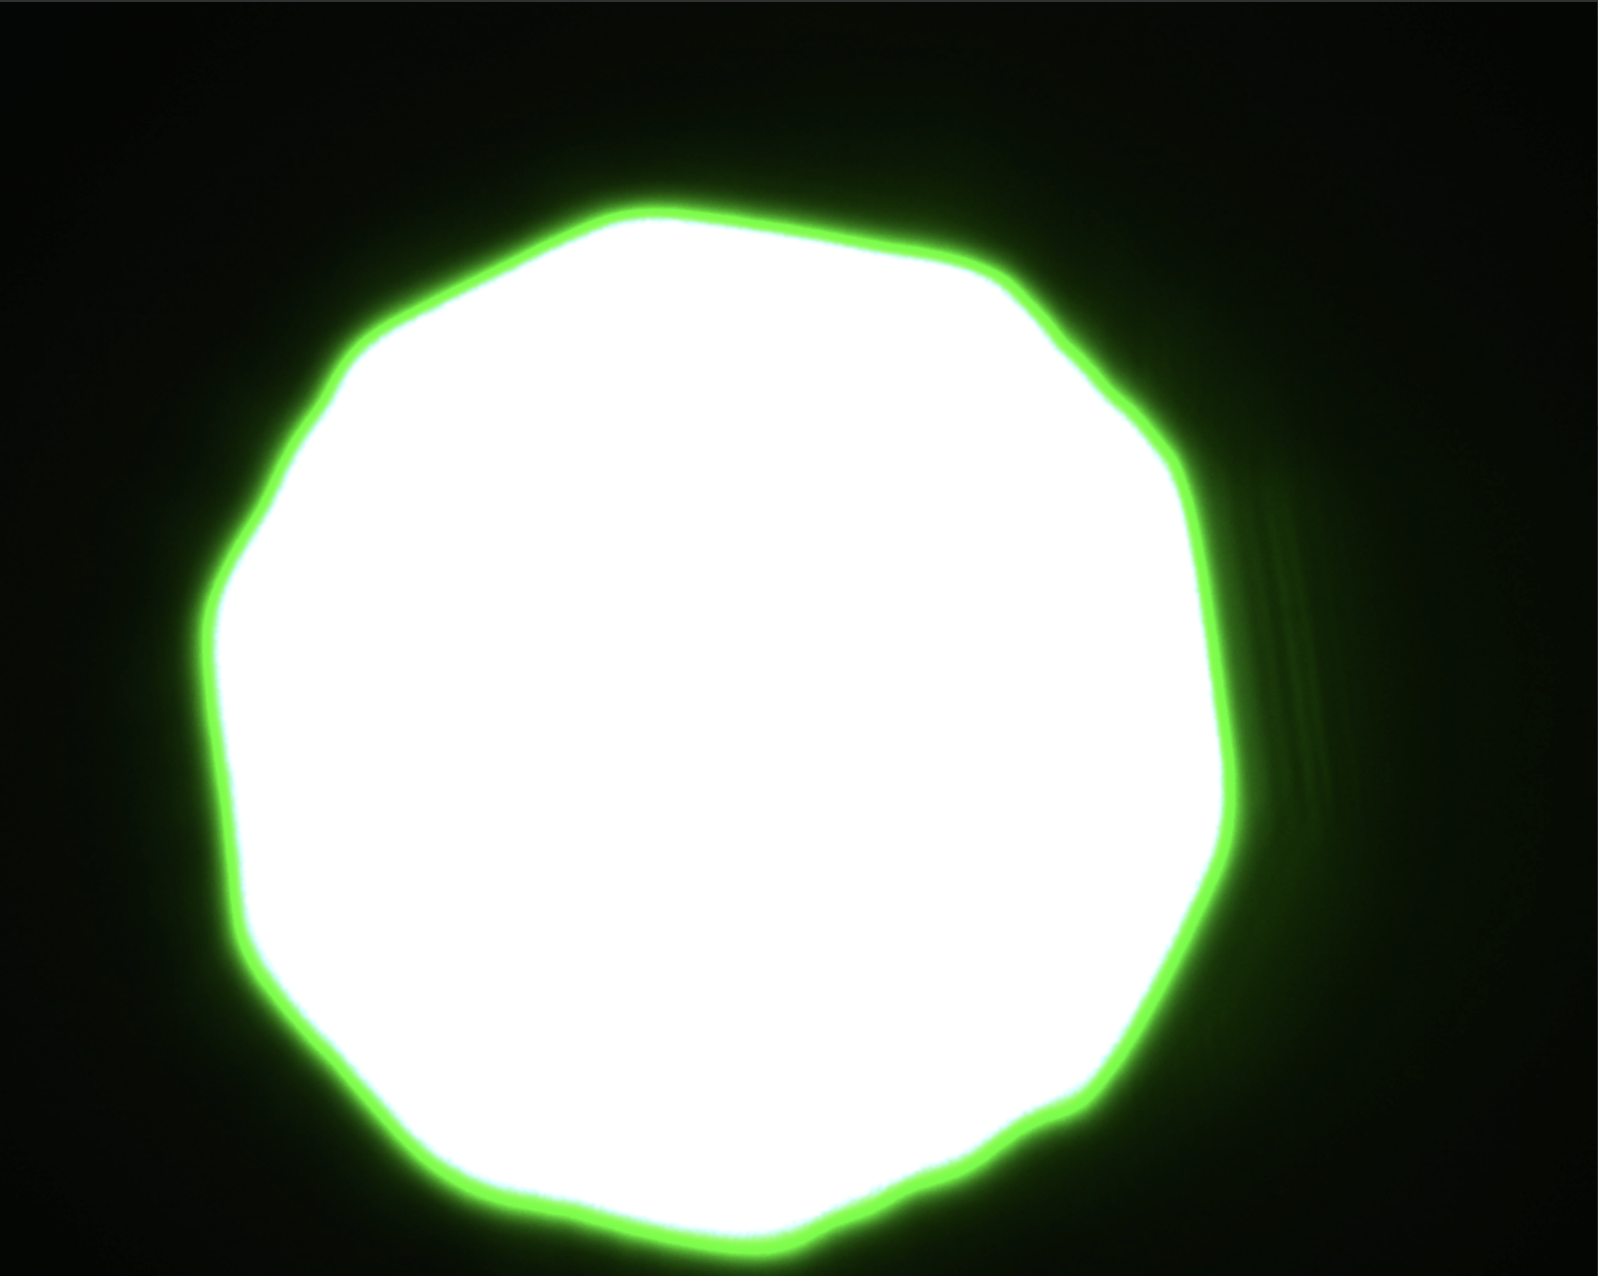
\includegraphics[width=\linewidth]{images/untitled_p5_img1.png}
\caption{F1 (\SI{4}{\micro\meter}).}
\end{subfigure}
\hfill
\begin{subfigure}[b]{0.46\textwidth}
\centering
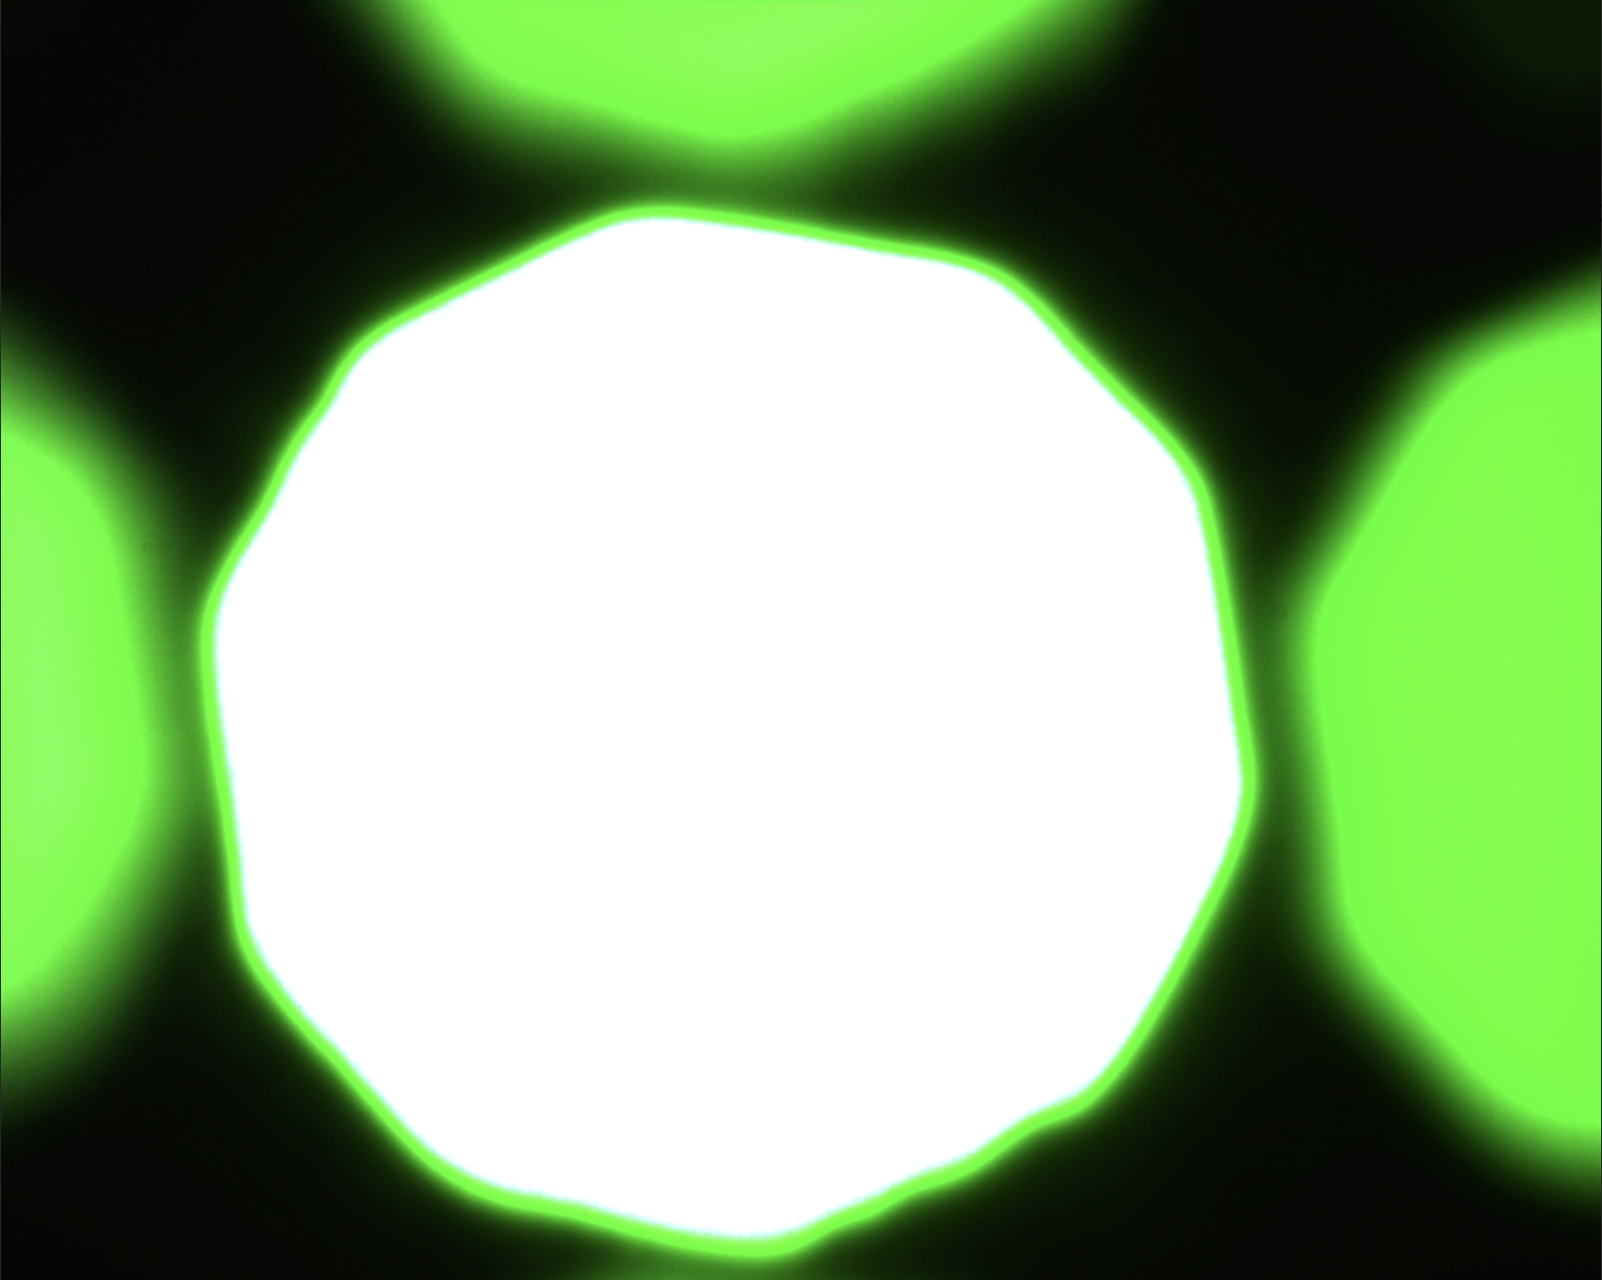
\includegraphics[width=\linewidth]{images/untitled_p5_img2.png}
\caption{F2 (\SI{6}{\micro\meter}).}
\end{subfigure}
\caption{Diffraction patterns for the Abbe-limit test (provided lab images). F1 shows stronger suppression of higher orders compared with F2, consistent with F1 lying at (or below) the predicted diffraction-limited separation while F2 lies above it.}
\label{fig:F1F2}
\end{figure*}

Figure~\ref{fig:F1F2} is consistent with the Abbe picture: a finite NA truncates the transmitted spatial-frequency spectrum. The \SI{4}{\micro\meter} target sits near the predicted cutoff, so higher diffraction orders are strongly attenuated (approaching an unresolved ``single-blob'' response), whereas the \SI{6}{\micro\meter} target transmits additional orders, producing visible side maxima.

\subsection{Experiment 3: bright-field vs dark-field diatom imaging}
\begin{figure*}[t]
\centering
\begin{subfigure}[b]{0.46\textwidth}
\centering
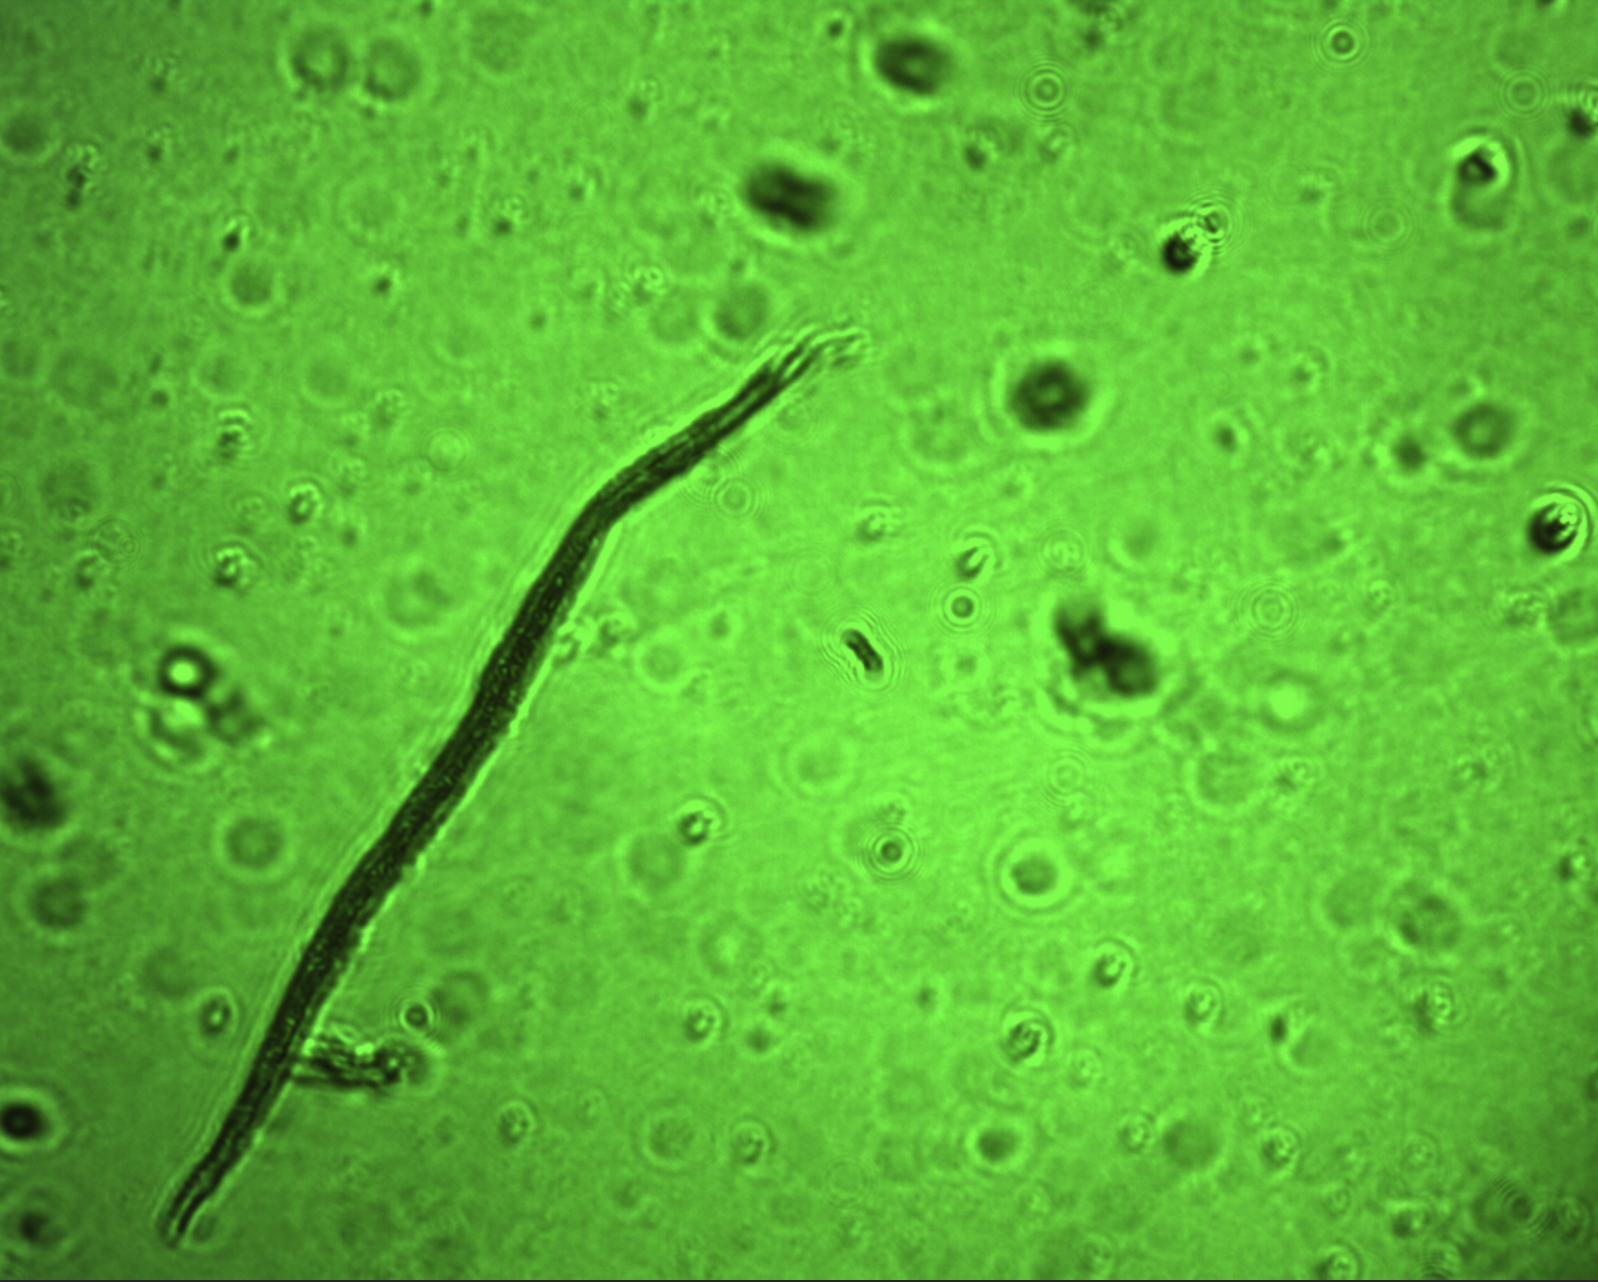
\includegraphics[width=\linewidth]{images/untitled_p6_img1.png}
\caption{Bright-field (no blocking).}
\end{subfigure}
\hfill
\begin{subfigure}[b]{0.46\textwidth}
\centering
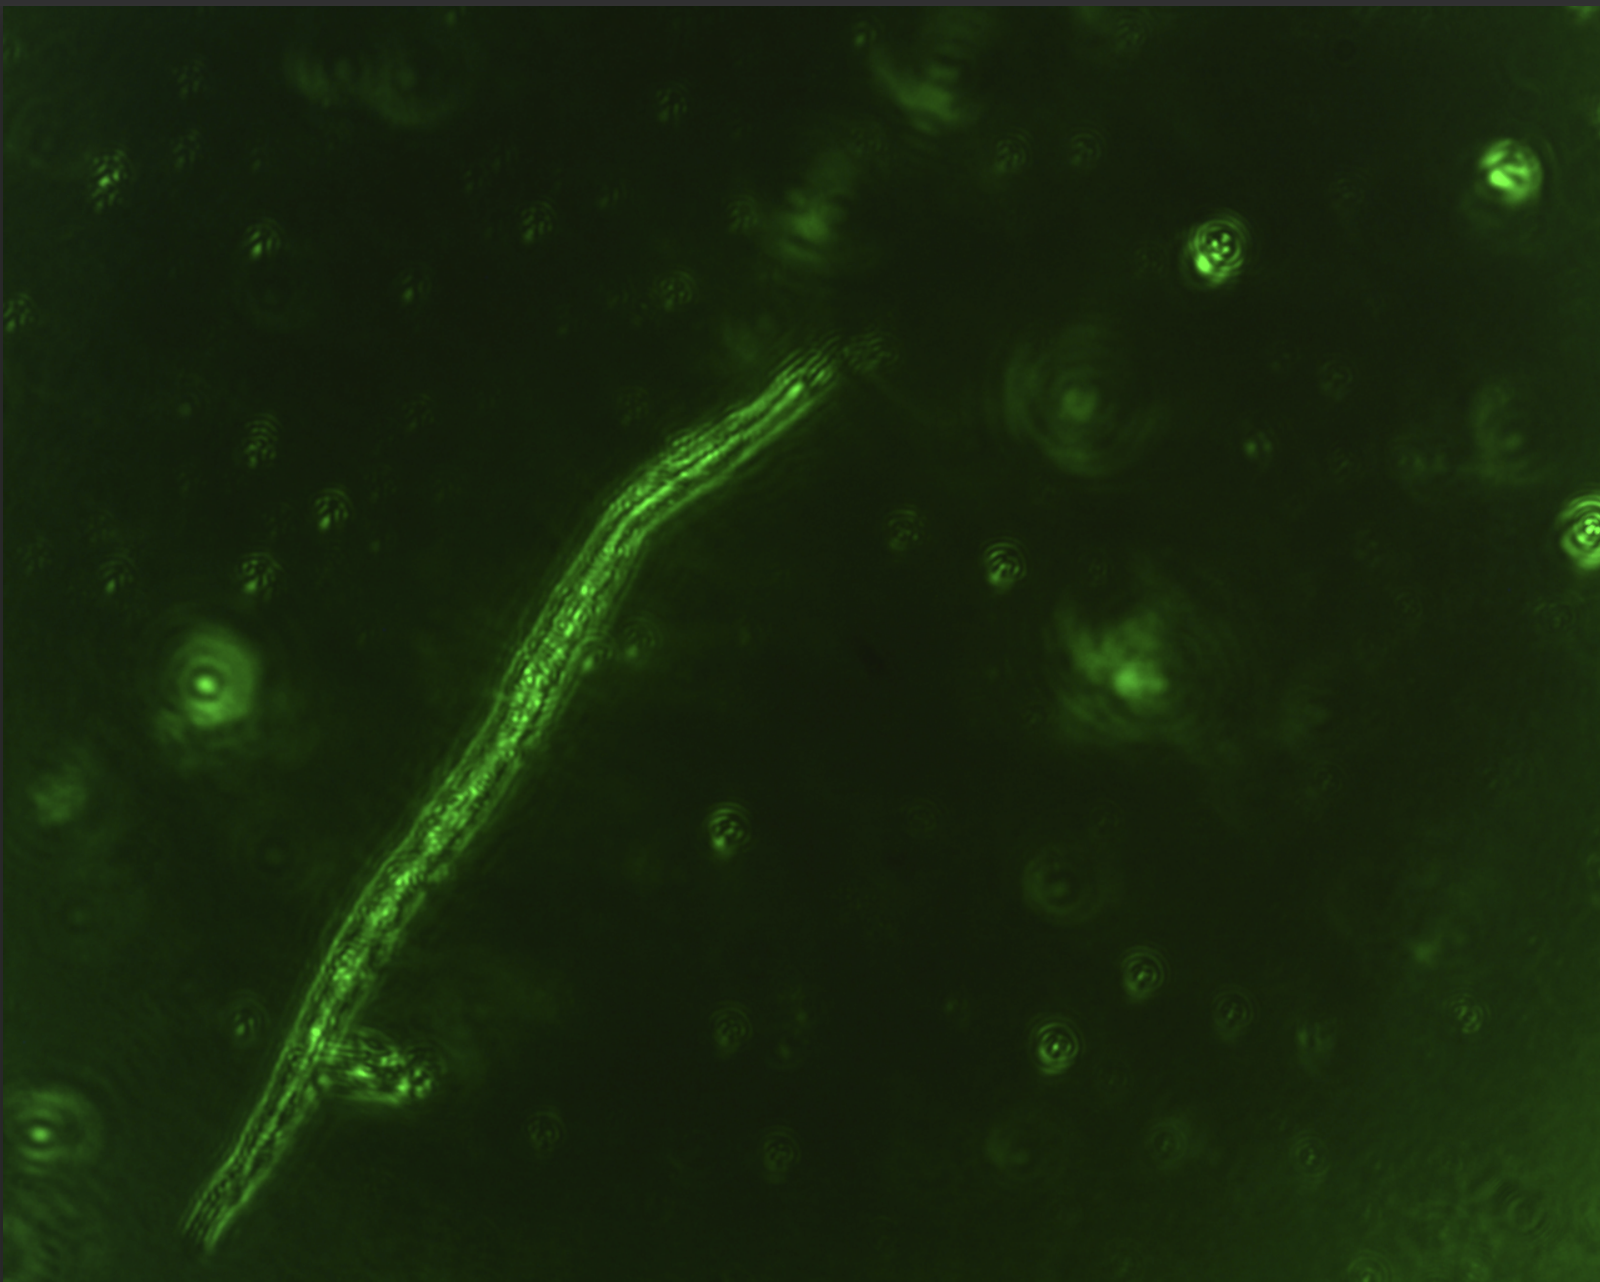
\includegraphics[width=\linewidth]{images/untitled_p6_img2.png}
\caption{Dark-field (zero order blocked).}
\end{subfigure}
\caption{Diatom specimen images (provided lab images). Blocking the Fourier-plane zero order suppresses the low-frequency background and highlights high-frequency features (edges/fine structure).}
\label{fig:diatom}
\end{figure*}

In bright-field (Fig.~\ref{fig:diatom}a) the image intensity is dominated by the undiffracted (DC) component, so weak phase/edge features appear with low contrast. In dark-field (Fig.~\ref{fig:diatom}b) blocking the zero order removes the background carrier and the image is formed primarily from scattered (higher spatial-frequency) components, so edges and fine structure become comparatively brighter.

\textbf{Electronics analogy.} Converting phase modulation into an amplitude/readout voltage in electronics is commonly done by \emph{coherent (phase-sensitive) detection}: mixing the signal with a phase-shifted reference (I/Q demodulation or a phase discriminator) converts relative phase into measurable amplitude in the baseband channels. The optical analogue is interference between a reference (zero-order) field and a scattered field; in dark-field the reference is removed, while in phase-contrast microscopy the reference is phase-shifted to convert phase variations into intensity.

\FloatBarrier
\section{Discussion: uncertainty budget, systematics, and improvements}
A compact comparison is given in Table~\ref{tab:compare} (Appendix). The camera method yields the smallest \emph{random} uncertainty (counting statistics + calibration pixel uncertainty) and, crucially, an explicit calibration chain. The screen-angle method is limited by geometric measurement of $y$ and spot size. The slit method's random uncertainty is small, but its total uncertainty is dominated by systematics:
\begin{itemize}
\item \textbf{Subjective threshold:} ``just-visible'' depends on observer, display gain, and how ``2D'' is defined.
\item \textbf{Slit centering:} an offset of the slit relative to the zero order changes which diffraction orders pass first, biasing $w_{\min}$ and therefore $d$.
\item \textbf{Wavelength (methods i \& iii only):} the green bandpass filter has finite bandwidth; using a single $\lambda=\SI{550}{\nano\meter}$ introduces a multiplicative scale systematic for the screen-angle and slit methods (both rely on $\lambda$). The calibrated-camera method is independent of $\lambda$ but inherits any systematic tolerance in the calibration target spacing.
\end{itemize}

\textbf{Concrete improvements (future work).} (i) Measure or narrow the illumination spectrum (spectrometer or narrower filter) to reduce the common wavelength systematic; (ii) replace subjective slit ``thresholding'' with an intensity-based criterion by recording Fourier-plane images as a function of $w$ and defining $w_{\min}$ at a fixed transmitted-order intensity fraction; (iii) quantify slit-centering systematics by deliberately scanning the slit laterally and fitting a model for the onset of first-order transmission; and (iv) turn Experiment~2 into a quantitative resolution study by sweeping the aperture iris (NA scan) and extracting a modulation transfer function (MTF) from line-pair targets.

\section{Conclusion and outlook}
We completed the three Fourier optics experiments specified in the EDU-FOP2 manual \S2.5. The grating period was measured as $d_{\mathrm{screen}}=\SI{9.87\pm0.26}{\micro\meter}$ and $d_{\mathrm{cam}}=\SI{9.92\pm0.11}{\micro\meter}$, consistent with the nominal \SI{10}{\micro\meter} scale; the slit cutoff method yielded $d_{\mathrm{slit}}=\SI{10.83\pm0.05}{\micro\meter}$ (random) but is best interpreted as systematics-dominated. Abbe's condition predicted $\Delta x_{\min}\approx\SI{4.0}{\micro\meter}$, consistent with the qualitative difference between F1 and F2 diffraction patterns. Finally, Fourier-plane zero-order blocking produced dark-field diatom images with markedly enhanced high-frequency contrast.

\textbf{Outlook.} The most impactful upgrades are (1) tighter control/measurement of $\lambda$, (2) objective, image-based definitions of slit cutoffs and diffraction-order visibility, and (3) NA-dependent resolution characterization (MTF extraction). Together these changes would convert the present demonstrations into a calibrated Fourier-microscopy benchmark suitable for publication-level characterization of spatial filtering and resolution.

\begin{thebibliography}{9}
\bibitem{thorlabs_manual}
Thorlabs, \emph{Fourier Optics Kit (EDU-FOP2) Manual}, Rev.\ B (Feb.\ 15, 2022).

\bibitem{ucsb_writeup}
PHYS 128AL Fourier Optics Lab Writeup (IPhO S24), Fourier-plane scaling and uncertainty relation discussion.
\end{thebibliography}

% ---------------------------------
% Appendices: raw data + full math
% ---------------------------------
\clearpage
\onecolumn
\appendix

\section{Raw data (with uncertainties)}
\label{app:raw}
\subsection{Experiment 1(i): screen geometry}
\begin{table}[H]
\centering
\caption{Screen-method raw data. Uncertainties are dominated by ruler placement and finite spot size. We conservatively assign $\sigma_L=\SI{0.1}{cm}$ and $\sigma_y=\SI{0.05}{cm}$ to reflect manual readout resolution.}
\label{tab:screenraw}
\begin{tabular}{@{}cccc@{}}
\toprule
Trial & $L$ (cm) & $y$ (cm) & Notes \\ \midrule
1 & 5  & 0.3 & 0th--1st order separation \\
2 & 8  & 0.4 & \\
3 & 12 & 0.7 & \\
4 & 18 & 1.0 & \\ \bottomrule
\end{tabular}
\end{table}

\subsection{Experiment 1(ii): camera calibration and counting}
\begin{table}[H]
\centering
\caption{Camera-calibration inputs. The \SI{0.74}{\milli\meter} spacing is the target specification; any manufacturing tolerance constitutes an additional systematic scale uncertainty not included in the random error propagation.}
\label{tab:cameraraw}
\begin{tabular}{@{}lc@{}}
\toprule
Quantity & Value \\ \midrule
Calibration spacing $\Delta x_{\rm obj}$ & \SI{0.74}{\milli\meter} \\
Pixels for $\Delta x_{\rm obj}$ & $1016\pm2$ px \\
Pixels used for grating count $N$ & $1280$ px \\
Grating periods counted $P$ & $94\pm1$ \\ \bottomrule
\end{tabular}
\end{table}

\subsection{Experiment 1(iii): slit cutoff}
\begin{table}[H]
\centering
\caption{Slit-method inputs. The quoted $\pm\SI{0.0005}{in}$ uncertainty reflects the knob tick size; the dominant uncertainty is systematic and is addressed in Appendix~\ref{app:calc} and the Discussion.}
\label{tab:slitraw}
\begin{tabular}{@{}lc@{}}
\toprule
Quantity & Value \\ \midrule
Objective focal length $f_{\rm obj}$ & \SI{30}{\milli\meter} \\
Wavelength $\lambda$ & \SI{550}{\nano\meter} (nominal) \\
Minimal slit width $w_{\min}$ & \SI{0.1200\pm0.0005}{in} \\ \bottomrule
\end{tabular}
\end{table}

\subsection{Experiment 2: Abbe criterion inputs}
\begin{table}[H]
\centering
\caption{Parameters used in the NA estimate (manual Eq.~36 implementation).}
\label{tab:abbeinputs}
\begin{tabular}{@{}lc@{}}
\toprule
Quantity & Value \\ \midrule
Aperture diameter $D$ & \SI{25.4}{\milli\meter} \\
Focal length $f$ & \SI{150}{\milli\meter} \\
Index $n$ & 1 (air) \\
Wavelength $\lambda$ & \SI{550}{\nano\meter} (nominal) \\
Test targets & F1: \SI{4}{\micro\meter}, F2: \SI{6}{\micro\meter} \\ \bottomrule
\end{tabular}
\end{table}

\section{Detailed calculations and uncertainty propagation}
\label{app:calc}
\subsection{Experiment 1(i): regression for $\tan\theta$}
We fit $y=mL$ (through-origin regression), so $m=\tan\theta$ and
\begin{equation}
 m = \frac{\sum_i L_i y_i}{\sum_i L_i^2}.
\end{equation}
Using Table~\ref{tab:screenraw} gives $m=0.0558$.

Using the four $(L_i,y_i)$ pairs in Table~\ref{tab:screenraw}, the key sums are
$\sum_i L_i^2=\SI{557}{cm^2}$ and $\sum_i L_i y_i=\SI{31.10}{cm^2}$, so
$m=\tan\theta=\sum_i L_i y_i/\sum_i L_i^2=0.05583$ and $\theta=\arctan m=0.05578\,\mathrm{rad}$.
Table~\ref{tab:screenres} lists the predicted values and residuals; the through-origin model gives
$R^2\simeq0.998$, indicating that a single small-angle $\theta$ is consistent with the data.

\begin{table}[H]
\centering
\caption{Diagnostics for the through-origin screen-angle regression $y=mL$. Residuals reflect finite spot size and ruler/marking uncertainty.}
\label{tab:screenres}
\begin{tabular}{@{}cccc@{}}
\toprule
$L$ (cm) & $y$ (cm) & $mL$ (cm) & $y-mL$ (cm) \\ \midrule
5  & 0.300 & 0.279 & 0.021 \\
8  & 0.400 & 0.447 & $-0.047$ \\
12 & 0.700 & 0.670 & 0.030 \\
18 & 1.000 & 1.005 & $-0.005$ \\ \bottomrule
\end{tabular}
\end{table}

 The standard error for a through-origin fit is
\begin{equation}
\sigma_m = \sqrt{\frac{1}{(N-1)\sum_i L_i^2}\sum_i (y_i-mL_i)^2},
\end{equation}
so $\sigma_\theta = \sigma_m/(1+m^2)$. For $d=\lambda/\sin\theta$,
\begin{equation}
\sigma_d = \left|\frac{\partial d}{\partial \theta}\right|\sigma_\theta
= \left|\frac{\lambda\cos\theta}{\sin^2\theta}\right|\sigma_\theta.
\end{equation}

\subsection{Experiment 1(ii): camera method uncertainty}

Numerically, $s=\SI{0.72835}{\micro\meter\,px^{-1}}$ and $\sigma_s/s=\sigma_{\Delta p}/\Delta p=2/1016=0.197\%$.
The dominant term is the discrete period count $\sigma_P/P=1/94=1.06\%$, so
\begin{equation}
\sigma_{d,\Delta p}\approx d\frac{\sigma_s}{s}=\SI{0.020}{\micro\meter},\qquad
\sigma_{d,P}\approx d\frac{\sigma_P}{P}=\SI{0.106}{\micro\meter},
\end{equation}
and $\sigma_d=\sqrt{\sigma_{d,\Delta p}^2+\sigma_{d,P}^2}=\SI{0.107}{\micro\meter}$.


With $s=\Delta x_{\rm obj}/\Delta p$ and $d=sN/P$,
\begin{equation}
\left(\frac{\sigma_d}{d}\right)^2 = \left(\frac{\sigma_s}{s}\right)^2 + \left(\frac{\sigma_P}{P}\right)^2,
\quad
\frac{\sigma_s}{s}=\frac{\sigma_{\Delta p}}{\Delta p}.
\end{equation}

\subsection{Experiment 1(iii): slit method and a simple systematic-bias model}

A useful consistency check is to ask what slit width would be required if the (wavelength-free) camera
result $d_{\rm cam}$ is taken as the best estimate of the true period:
\begin{equation}
w_{\rm true}=\frac{2f\lambda}{d_{\rm cam}}=\SI{3.33}{\milli\meter}=\SI{0.131}{in},
\end{equation}
whereas we recorded $w_{\min}=\SI{3.048}{\milli\meter}=\SI{0.120}{in}$. The difference
$\Delta w\simeq\SI{0.28}{\milli\meter}=\SI{0.011}{in}$ corresponds to a $\sim9\%$ under-estimate of
$w_{\min}$, which is entirely plausible for a subjective ``just-visible'' criterion.

If the slit is laterally mis-centered by $\delta$ so that one first-order lobe passes when $w/2\approx x_1-\delta$
(with $x_1=f\lambda/d$), then $w_{\min}$ is biased low by $2\delta$ and
\begin{equation}
\frac{d_{\rm est}}{d_{\rm true}}\approx\frac{1}{1-\delta/x_1}.
\end{equation}
For $d_{\rm true}\approx d_{\rm cam}$ we have $x_1=f\lambda/d_{\rm cam}\approx\SI{1.66}{\milli\meter}$, so
$\delta\approx\Delta w/2\simeq\SI{0.14}{\milli\meter}$ would explain the observed $\sim\SI{0.9}{\micro\meter}$
offset of the slit method.


From $d=2f\lambda/w$, the random error from the micrometer tick size is $\sigma_d/d\approx\sigma_w/w$. However, if the slit is offset from the zero order by $\delta$, the onset condition becomes $w/2+\delta\approx x_1$. Solving for $d$,
\begin{equation}
 d_{\rm eff} \approx \frac{f\lambda}{w/2+\delta},
\end{equation}
so even modest mis-centering biases $d$.


\subsection{Common scale systematics and an ``overall'' budget}
For methods that depend on $\lambda$ (screen-angle and slit cutoff), the period scales linearly with the effective
illumination wavelength. The EDU-FOP2 kit uses a green bandpass filter centered at \SI{550}{\nano\meter} with
FWHM \SI{40}{\nano\meter}; without an independent spectral measurement, a conservative \emph{systematic} wavelength
uncertainty can be bounded at the $\pm\SI{20}{\nano\meter}$ half-width. If we approximate the unknown effective
$\lambda$ as uniformly distributed across this half-width, a $1\sigma$ uncertainty is
$\sigma_\lambda \approx 20/\sqrt{3}\,\si{\nano\meter}\approx\SI{11.5}{\nano\meter}$, i.e.\ a \SI{2.1}{\percent}
multiplicative systematic. This contributes $\sim\SI{0.21}{\micro\meter}$ to $d_{\rm screen}$ and
$\sim\SI{0.23}{\micro\meter}$ to $d_{\rm slit}$, comparable to (or larger than) their random components.

The calibrated-camera method does \emph{not} depend on $\lambda$, but it inherits any tolerance in the nominal
\SI{0.74}{\milli\meter} target spacing and any residual geometric distortion. If the target spacing has a fractional
tolerance $\epsilon_{\rm cal}$, then $d_{\rm cam}$ inherits the same systematic: $\sigma_{d,{\rm cal}} \approx \epsilon_{\rm cal} d$.

\begin{table}[H]
\centering
\caption{Summary uncertainty budget for Experiment~1. Random uncertainties are propagated from the recorded data.
Systematic terms are either estimated (wavelength bandwidth) or parameterized (camera calibration tolerance).}
\label{tab:ubudget}
\begin{tabular}{@{}lccc@{}}
\toprule
Method & $d$ (\si{\micro\meter}) & $\sigma_{\rm rand}$ (\si{\micro\meter}) & Key systematics \\ \midrule
Screen-angle & 9.87 & 0.26 & $\lambda$ bandwidth: $\sim$2.1\% ($\sim$0.21) \\
Camera (calibrated) & 9.92 & 0.11 & calibration spacing tolerance: $\epsilon_{\rm cal}\,d$ \\
Slit cutoff & 10.83 & 0.05 & threshold/centering bias: $\Delta w\simeq0.28$ mm ($\Rightarrow \Delta d\simeq0.9$) \\
\bottomrule
\end{tabular}
\end{table}

\subsection{Experiment 2: NA and $\Delta x_{\min}$}
With $\sin\alpha\approx D/(2f)$,
\begin{equation}
\mathrm{NA}\approx\frac{D}{2f},\qquad
\Delta x_{\min}=0.61\,\frac{\lambda}{\mathrm{NA}}.
\end{equation}

\clearpage
\section{Supplementary table: comparison of methods}
\begin{table}[H]
\centering
\caption{Comparison of grating period measurements and relative \emph{random} uncertainties. The slit method's quoted random uncertainty is not representative of its total uncertainty because the dominant error is systematic (centering + threshold definition).}
\label{tab:compare}
\begin{tabular}{@{}lccc@{}}
\toprule
Method & Result $d$ (\si{\micro\meter}) & $\sigma_d$ (\si{\micro\meter}) & $\sigma_d/d$ \\ \midrule
Screen diffraction angle & 9.87 & 0.26 & 2.6\% \\
Calibrated camera image & 9.92 & 0.11 & 1.1\% \\
Fourier-plane slit cutoff & 10.83 & 0.05 & 0.4\% (random) \\ \bottomrule
\end{tabular}
\end{table}

\end{document}
